\section{Results}
\label{sec:results}
We report fingerprinting performance at the family, architecture, and variant
levels, then for short observation windows and under a size-padding defense.
Scores are balanced accuracy, for which chance is $1/|\mathcal{C}|$.

\subsection{Family Identification}
Table~\ref{tab:family_methods} compares family identification methods. Under the
repeated protocol used for the earlier methods (20 seeds $\times$ 5-fold
model-disjoint cross-validation), the cross-device representation
of~\eqref{eq:crossdevice} achieves $0.68 \pm 0.04$, the highest among all
methods evaluated this way (fixed late fusion: 0.61) and 0.20 above a per-client
random forest ($0.48 \pm 0.04$). Under leave-one-model-out validation, which
trains on all remaining models, it reaches 0.74 (95\% CI 0.58--0.88, macro F1
0.74), significantly above chance (permutation test, $p = 0.003$), compared with
0.58 for the per-client random forest. Recurrent networks are identified without
error (6/6), convolutional networks in 7 of 9 cases, autoencoders in 6 of 9, and
transformers in 4 of 8 (Fig.~\ref{fig:family_confusion}). The remaining errors
involve architectures whose compute per parameter overlaps.

\begin{table}[!htbp]
\centering
\caption{Family Identification (4 classes, chance 0.25)}
\label{tab:family_methods}
\scriptsize
\renewcommand{\arraystretch}{1.08}
\setlength{\tabcolsep}{3pt}
\begin{tabular}{lcc}
\hline
 & \multicolumn{2}{c}{\textbf{Balanced accuracy}} \\
\textbf{Method} & \textbf{Repeated CV} & \textbf{Leave-one-model-out} \\
\hline
306-feature morphology (RF)        & 0.55 & -- \\
Compute-per-byte                   & 0.57 & -- \\
Fixed late fusion                  & 0.61 & -- \\
Equal-probability hybrid fusion    & 0.68$^{*}$ & -- \\
Per-client RF                      & 0.48 & 0.58 \\
\textbf{Cross-device LR (proposed)} & \textbf{0.68} & \textbf{0.74} \\
\hline
\end{tabular}

\vspace{2pt}
\parbox{0.95\columnwidth}{\scriptsize Repeated CV: mean over 20 seeds
$\times$ 5-fold model-disjoint cross-validation. Leave-one-model-out: nested
selection, 95\% CI 0.58--0.88 for the proposed method. $^{*}$Single 5-fold run.}
\end{table}

\begin{figure}[!t]
\centering
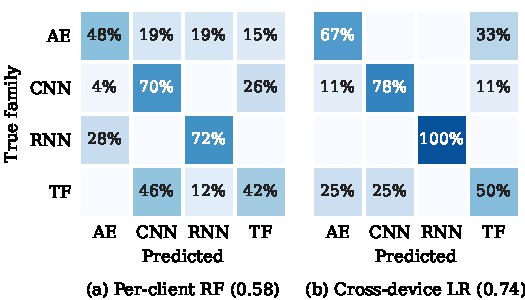
\includegraphics[width=\columnwidth]{fig_family_before_after.pdf}
\caption{Family confusion matrices for (a) the per-client baseline and (b) the
cross-device representation (leave-one-model-out). Cells give the percentage of
each true family assigned to each predicted family; empty cells are zero.
Balanced accuracy in parentheses.}
\label{fig:family_confusion}
\end{figure}

\subsection{Architecture Identification}
Using packet-morphology features, the architecture is identified within each
family well above chance (Table~\ref{tab:architecture_methods}). Recurrent architectures are separated
perfectly (1.00), autoencoder architectures reach 0.89, and convolutional
architectures 0.78. Transformer architectures are the most difficult (0.47),
partly because DistilBERT is represented by a single model. The mean across
families is 0.79 (macro F1 0.78), and the cross-device representation raises
convolutional architectures further to 0.81.

\begin{table}[!htbp]
\centering
\caption{Architecture Identification Within Each Family (Balanced Accuracy)}
\label{tab:architecture_methods}
\scriptsize
\renewcommand{\arraystretch}{1.08}
\setlength{\tabcolsep}{3pt}
\begin{tabular}{lccccc}
\hline
\textbf{Method} & \textbf{AE} & \textbf{CNN} & \textbf{RNN} & \textbf{Transf.} & \textbf{Mean} \\
\hline
Per-client RF (packet) & \textbf{0.89} & 0.78 & \textbf{1.00} & \textbf{0.47} & \textbf{0.79} \\
Cross-device LR & 0.67 & \textbf{0.81} & \textbf{1.00} & 0.25 & 0.68 \\
\hline
Chance          & 0.33 & 0.33 & 0.50 & 0.33 & -- \\
\hline
\end{tabular}
\end{table}

\subsection{Variant Identification}
At the finest level of the hierarchy, the uploaded payload size provides a
baseline leak. It is recovered from traffic within a median relative error of
$0.025\%$ of the true serialized size. Because every variant has a distinct
size, nearest-reference matching identifies the exact variant in all 90 traces
(chance $3.4\%$). Table~\ref{tab:variant_results} summarizes
the result per family.
Accounting for the client-specific header length is essential: assuming a single
header length under-counts the Windows client's payload by $0.8\%$ and causes
three of the 90 identifications to fail. Within a 5~s window, every variant with a short download is
identified, including all recurrent networks, autoencoders, MobileNets, and Tiny
Transformers, whereas EfficientNet, ResNet, and larger BERT downloads exceed the
window.

\begin{table}[!htbp]
\centering
\caption{Variant Identification by Payload Size}
\label{tab:variant_results}
\scriptsize
\renewcommand{\arraystretch}{1.05}
\setlength{\tabcolsep}{3pt}
\begin{tabular}{lcccc}
\hline
\textbf{Family} & \textbf{Traces} & \textbf{Payload (MB)} & \textbf{Trace} & \textbf{5~s} \\
\hline
Autoencoder & 27 & 0.01--10.1  & 1.00 & 0.96 \\
CNN         & 24 & 6.2--170.7  & 1.00 & 0.25 \\
RNN         & 18 & 0.22--2.2   & 1.00 & 1.00 \\
Transformer & 21 & 6.8--373.8  & 1.00 & 0.57 \\
\hline
\textbf{Total} & \textbf{90} & & \textbf{1.00} & \textbf{0.69} \\
\hline
\end{tabular}

\vspace{2pt}
\parbox{0.95\columnwidth}{\scriptsize Nearest-reference matching on log payload
size; 5~s: one complete download within a 5~s window. ResNet-34 and DistilBERT
are excluded (incomplete capture).}
\end{table}

\subsection{Discriminative Features}
\label{subsec:features}
Fisher scores computed on all observations indicate which features drive each
task; during evaluation, features are selected within each training fold. Transmission rates separate
families in per-client traces, whereas the cross-device representation relies on
burst and packet-size dispersion, led by the laptop's view of the same model.
The compute-timing features rank first for architecture identification in three
of the four families, through the compute gap per megabyte for autoencoders and
the cross-device gap ratio for recurrent networks and transformers.


\subsection{Short Observation Windows}
Table~\ref{tab:window_results} reports all three levels for single windows of
0.5 to 5~s and for longer observation times of 10 to 30~s. For family identification, single-client windows reach only 0.26--0.31 per
window, whereas concatenating the three clients' time-aligned windows, removing
near-idle windows, and classifying with logistic regression reaches 0.41 per
window at 0.5~s, rising to 0.51 at 5~s, and 0.51--0.65 after averaging window
posteriors per experiment. The cross-device gain is consistent across all window
sizes. The same representation identifies convolutional architectures with
0.65--0.71 per window and 0.89 after pooling at every window size, and
autoencoder architectures with up to 0.78 after pooling; recurrent and
transformer architectures, each represented by few models, are not reliably
identifiable from short windows. Variant identification requires a complete
model transfer within the window. Because model downloads are faster than
uploads on the testbed, a window that begins at a download identifies the exact
variant in $23\%$ of traces at 0.5~s, rising to $69\%$ at 5~s, and identifies
it correctly whenever the download completes within the window.

\begin{table}[!htbp]
\centering
\caption{Accuracy Versus Observation Time}
\label{tab:window_results}
\scriptsize
\renewcommand{\arraystretch}{1.08}
\setlength{\tabcolsep}{2pt}
\begin{tabular}{lcccc|cccc}
\hline
& \multicolumn{4}{c|}{\textbf{Single window}} & \multicolumn{4}{c}{\textbf{Accumulated}} \\
\textbf{Task} & \textbf{0.5~s} & \textbf{1~s} & \textbf{2~s} & \textbf{5~s} & \textbf{10~s} & \textbf{15~s} & \textbf{20~s} & \textbf{30~s} \\
\hline
Family, single client     & 0.26 & 0.29 & 0.30 & 0.31 & 0.31 & 0.31 & 0.30 & 0.30 \\
\textbf{Family, cross-device} & \textbf{0.41} & \textbf{0.43} & \textbf{0.46} & \textbf{0.51} & \textbf{0.53} & \textbf{0.54} & \textbf{0.55} & \textbf{0.56} \\
\hline
Arch., autoencoder         & 0.50 & 0.52 & 0.45 & 0.47 & 0.48 & 0.48 & 0.48 & 0.47 \\
Arch., CNN                 & 0.65 & 0.67 & 0.69 & 0.71 & 0.76 & 0.78 & 0.80 & 0.81 \\
Arch., RNN                 & 0.54 & 0.51 & 0.39 & 0.35 & 0.29 & 0.29 & 0.27 & 0.28 \\
Arch., transformer         & 0.21 & 0.22 & 0.20 & 0.19 & 0.20 & 0.19 & 0.19 & 0.19 \\
\hline
Variant$^{\dagger}$        & 0.23 & 0.32 & 0.39 & 0.69 & 0.80 & 0.82 & 0.86 & 0.90 \\
\hline
\end{tabular}

\vspace{2pt}
\parbox{0.95\columnwidth}{\scriptsize Balanced accuracy per decision. Family and
architecture: cross-device LR with near-idle windows removed, experiment-disjoint
5-fold CV grouped by model; 10--30~s average the posteriors of consecutive 5~s
windows over non-overlapping spans. Chance 0.25 (family), 0.33 (autoencoder,
CNN, transformer), 0.50 (RNN). $^{\dagger}$Share of traces whose variant is
identified from one complete download within the observation time.}
\end{table}

Accumulating evidence over longer observation helps where the per-window signal
is consistent (Table~\ref{tab:window_results}). Averaging the posteriors of
consecutive 5~s windows raises cross-device family accuracy from 0.51 at 5~s to
0.56 at 30~s and convolutional architecture accuracy from 0.71 to 0.81, whereas
the single-client baseline remains at 0.30--0.31 and autoencoder architecture
does not improve. Variant identification, which depends on capturing a complete
download, rises from $69\%$ of traces at 5~s to $90\%$ at 30~s.


\subsection{Ablation}
\label{subsec:ablation}
Table~\ref{tab:ablation} isolates the components of the proposed model under the
same leave-one-model-out protocol with nested selection. Neither component helps
in isolation: the cross-device representation with a random forest reaches 0.45,
and a per-client logistic regression also reaches 0.45, both below the per-client
random forest (0.58). Combined, they reach 0.74. Concatenating the three devices
yields few high-dimensional examples, which tree ensembles overfit but a
regularized linear model exploits. The compute-timing features contribute a
further 0.15 (0.59 without them). For short windows, the cross-device
representation improves both classifiers (5~s per-window accuracy from 0.31 to
0.44 with a random forest and from 0.35 to 0.49 with logistic regression), and
removing near-idle windows adds 0.02 per window. The cross-device gain does not
depend on a single device: with the laptop removed, combining the remaining two
devices still reaches 0.71 (95\% CI 0.57--0.85). As an upper bound, excluding
the ten variants whose compute profiles overlap another family (for example,
large ResNet and BERT models) and re-evaluating the round-level features on the
remaining 19 models raises nested leave-one-model-out family accuracy to 0.85;
because these exclusions were chosen from the observed errors, this figure bounds
the achievable accuracy rather than estimating generalization.

\begin{table}[!htbp]
\centering
\caption{Ablation of the Family Model (Balanced Accuracy)}
\label{tab:ablation}
\scriptsize
\renewcommand{\arraystretch}{1.08}
\setlength{\tabcolsep}{3pt}
\begin{tabular}{llccc}
\hline
\textbf{Representation} & \textbf{Classifier} & \textbf{Comp.} & \textbf{Bal. acc.} & \textbf{95\% CI} \\
\hline
\multicolumn{5}{l}{\textit{Complete trace (leave-one-model-out)}} \\
Per-client   & RF & \checkmark & 0.58 & 0.42--0.74 \\
Per-client   & LR & \checkmark & 0.45 & 0.34--0.56 \\
Cross-device & RF & \checkmark & 0.45 & 0.27--0.64 \\
Cross-device & LR & --         & 0.59 & 0.45--0.75 \\
\textbf{Cross-device} & \textbf{LR} & \checkmark & \textbf{0.74} & 0.58--0.88 \\
\hline
\multicolumn{5}{l}{\textit{5~s windows, per window / pooled}} \\
Single-client & RF & -- & \multicolumn{2}{c}{0.31 / 0.31} \\
Single-client & LR & -- & \multicolumn{2}{c}{0.35 / 0.40} \\
Cross-device  & RF & -- & \multicolumn{2}{c}{0.44 / 0.45} \\
Cross-device  & LR & -- & \multicolumn{2}{c}{0.49 / 0.62} \\
\textbf{Cross-device}$^{\dagger}$ & \textbf{LR} & -- & \multicolumn{2}{c}{\textbf{0.51 / 0.62}} \\
\hline
\end{tabular}

\vspace{2pt}
\parbox{0.95\columnwidth}{\scriptsize Comp.: compute-timing features.
$^{\dagger}$Near-idle windows removed. Windows: experiment-disjoint 5-fold CV
grouped by model.}
\end{table}

\subsection{Robustness to Size Padding}
\label{subsec:padding}
Padding every transfer to a size bucket defeats variant identification:
accuracy falls from 1.00 to 0.60 with 1~MB buckets ($1.8\%$ byte overhead),
to 0.45 with power-of-two buckets ($47\%$), and to chance (0.03) when all
transfers are padded to the largest model, at $1{,}086\%$ overhead. Family identification is unaffected, because the
compute gap and cross-device timing ratios do not depend on transfer size: using
these timing features alone, cross-device family identification reaches 0.62
(95\% CI 0.45--0.78, $p = 0.005$), matching the same model with size features
(0.60). Concealing model identity therefore requires timing defenses in addition
to size padding.


\subsection{Summary}
The cross-device timing signature reveals the family of unseen models (0.74),
also from short windows (0.51 per 5~s window, where it also identifies
convolutional architectures with 0.71), and remains effective under padding
(0.62). Within a family, packet-morphology features identify the architecture
with a mean balanced accuracy of 0.79. Payload size reveals the exact variant
(1.00, and 0.69 from a single download within a 5~s window), although padding
removes this signal.
